%% agentic-coding-diff.tex: the anatomy of a unified diff (Chapter 5).
%% Not a house concept diagram but an annotated listing: the left column is a
%% minimal unified-diff hunk, one line per row; the right column names each
%% structural element (file lines, hunk header, context, removed, added) with a
%% terse label joined by a dotted leader, and the caption carries the gloss.
%% Palette follows the +/- convention: added green, removed red, context grey.
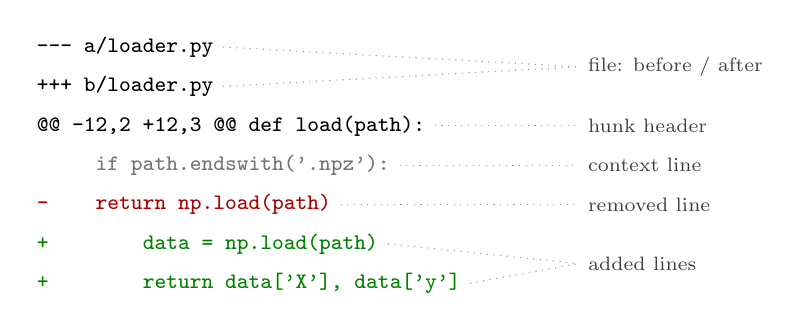
\begin{tikzpicture}[
  diffline/.style={font=\footnotesize\ttfamily, anchor=west},
  role/.style={font=\scriptsize, anchor=west, text=black!75},
  lead/.style={dotted, black!40},
]
% left column: the diff hunk, top to bottom
\node[diffline]                     (l1) at (0, 0.0)  {-{}-{}- a/loader.py};
\node[diffline]                     (l2) at (0,-0.5)  {+++ b/loader.py};
\node[diffline]                     (l3) at (0,-1.0)  {@@ -12,2 +12,3 @@ def load(path):};
\node[diffline, text=black!55]      (l4) at (0,-1.5)  {\ \ \ \ \ if path.endswith('.npz'):};
\node[diffline, text=red!65!black]  (l5) at (0,-2.0)  {-\ \ \ \ return np.load(path)};
\node[diffline, text=green!50!black](l6) at (0,-2.5)  {+\ \ \ \ \ \ \ \ data = np.load(path)};
\node[diffline, text=green!50!black](l7) at (0,-3.0)  {+\ \ \ \ \ \ \ \ return data['X'], data['y']};

% right column: terse role labels
\node[role] (a) at (7.0,-0.25) {file: before / after};
\node[role] (b) at (7.0,-1.0)  {hunk header};
\node[role] (c) at (7.0,-1.5)  {context line};
\node[role] (d) at (7.0,-2.0)  {removed line};
\node[role] (e) at (7.0,-2.75) {added lines};

% dotted leaders from each element to its label
\draw[lead] (l1.east) -- (a.west);
\draw[lead] (l2.east) -- (a.west);
\draw[lead] (l3.east) -- (b.west);
\draw[lead] (l4.east) -- (c.west);
\draw[lead] (l5.east) -- (d.west);
\draw[lead] (l6.east) -- (e.west);
\draw[lead] (l7.east) -- (e.west);
\end{tikzpicture}%
